\section{Implementierung}
\label{sec:implementation}
\subsection{List-based set with coarse-grained locks}

Bei dieser Implementierung wir vor jedem Methodenaufruf die gesamte Liste gesperrt. Dadurch kann aber die Parallelisierung nicht wirklich ausgenutzt werden, da zu einem Zeitpunkt maximal ein Prozess auf die Liste zugreifen kann. Diese Implementierung ist daher sehr ähnlich zu einer sequentiellen Implementierung.

\begin{figure}[H]
	\centering
    \begin{tikzpicture}
        \draw (-0.5,1) -- (10.5,1) node [midway, above, sloped] {\faLock};
		\node[draw,circle,minimum size=1cm,inner sep=0pt] at (0,0) {$- \infty$};
		\draw[->] (0.5,0) -- (1.5,0);
		\node[draw,circle,minimum size=1cm,inner sep=0pt] at (2,0) {$3$};
		\draw[->] (2.5,0) -- (3.5,0);
		\node[draw,circle,minimum size=1cm,inner sep=0pt] at (4,0) {$5$};
		\draw[->] (4.5,0) -- (5.5,0);
		\node[draw,circle,minimum size=1cm,inner sep=0pt] at (6,0) {$8$};
		\draw[->] (6.5,0) -- (7.5,0);
		\node[draw,circle,minimum size=1cm,inner sep=0pt] at (8,0) {$10$};
		\draw[->] (8.5,0) -- (9.5,0);
		\node[draw,circle,minimum size=1cm,inner sep=0pt] at (10,0) {$\infty$};
	\end{tikzpicture}
	\caption{coarse-grained locks}
	\label{tik:coarse-grained}
\end{figure}

\begin{table}[H]
    \begin{tabularx}{\textwidth}{lX}
        \textit{add} & Nachdem die Liste gesperrt wurde wird sie durchlaufen bis zu dem Punkt an dem der Key der betrachteten Node größer ist als der Einzufügende. Vor dieser wird die Neue Node eingefügt. \\
        \textit{contains} & Die Liste wird gesperrt und dann durchlaufen. Wenn dabei der gesuchten Wert gefunden wird, wird \textit{true} sont \textit{false} zurückgegeben.\\
        \textit{remove} & Nachdem die gesamte Liste gesperrt wurde wird das Element in der Liste gesucht und entfernt.\\
    \end{tabularx}
\end{table}

\subsection{List-based set with fine-grained locks}

Im Unterschied zu den coarse-grained locks wird bei dieser Implementierung immer nur die derzeitige Node gesprerrt. 
Beim Iterieren der Liste wird während dem Übergang zur nächsten Node die derzeitige und die darauffolgende Node gesperrt. 
Eine Node kann zu einem Zeitpunkt nur von einem Prozess gesperrt sein. Der Vorteil gegenüber den coarse-grained locks besteht darin, 
dass nun wirkliche Parallelisierung möglich ist und verschiedene Threads an unterschiedlichen Punkten an der Liste arbeiten können. 
Es hat jedoch den Nachteil, dass die Iterationsgeschwiendigkeit im Worst Case durch den langsamsten Thread definiert wird, da ein 
Thread in der Liste nicht ``Überholt'' werden kann.

\begin{figure}[H]
	\centering
    \begin{tikzpicture}
        \draw (3.5,1) -- (4.5,1) node [midway, above, sloped] {\faLock};
        \draw (5.5,1) -- (6.5,1) node [midway, above, sloped] {\faLock};
		\node[draw,circle,minimum size=1cm,inner sep=0pt] at (0,0) {$- \infty$};
		\draw[->] (0.5,0) -- (1.5,0);
		\node[draw,circle,minimum size=1cm,inner sep=0pt] at (2,0) {$3$};
		\draw[->] (2.5,0) -- (3.5,0);
		\node[draw,circle,minimum size=1cm,inner sep=0pt] at (4,0) {$5$};
		\draw[->] (4.5,0) -- (5.5,0);
		\node[draw,circle,minimum size=1cm,inner sep=0pt] at (6,0) {$8$};
		\draw[->] (6.5,0) -- (7.5,0);
		\node[draw,circle,minimum size=1cm,inner sep=0pt] at (8,0) {$10$};
		\draw[->] (8.5,0) -- (9.5,0);
		\node[draw,circle,minimum size=1cm,inner sep=0pt] at (10,0) {$\infty$};
	\end{tikzpicture}
	\caption{fine-grained locks}
	\label{tik:fine-grained}
\end{figure}

\begin{figure}[H]
	\centering
    \begin{tikzpicture}
        \draw (3.5,1) -- (4.5,1) node [midway, above, sloped] {\faLock};
        \draw (5.5,-1) -- (6.5,-1) node [midway, above, sloped] {\faLock};
		\node[draw,circle,minimum size=1cm,inner sep=0pt] at (0,0) {$- \infty$};
		\draw[->] (0.5,0) -- (1.5,0);
		\node[draw,circle,minimum size=1cm,inner sep=0pt] at (2,0) {$3$};
		\draw[->] (2.5,0) -- (3.5,0);
		\node[draw,circle,minimum size=1cm,inner sep=0pt] at (4,0) {$5$};
        \draw[->] (4.5,0) -- (7.5,0);
        \draw[line width=0.5mm, red] (5.5,-1.5) -- (6.5,-2.5);
        \node[draw,circle,minimum size=1cm,inner sep=0pt] (A) at (6,-2) {$8$};
        \node[draw,circle,minimum size=1cm,inner sep=0pt] (B) at (8,0) {$10$};
        \draw[->] (A) -- (B);
		\draw[->] (8.5,0) -- (9.5,0);
		\node[draw,circle,minimum size=1cm,inner sep=0pt] at (10,0) {$\infty$};
	\end{tikzpicture}
	\caption{fine-grained locks remove}
	\label{tik:fine-grained-remove}
\end{figure}

\begin{table}[H]
    \begin{tabularx}{\textwidth}{lX}
        \textit{add} & Die Liste wird iteriert (mit Sperrungen) und an dem Punkt an dem die Node eingefügt werden soll wird sowohl der Vorgänger als auch der Nachfolger gesperrt. Dadurch kann die neue Node sicher eingefügt werden.\\
        \textit{contains} & Die Liste wird analog zur coarse-grained locks iteriert dabei aber immer die derzeitige Node bzw. beim Übergang Vorgänger und Nachfolger gesperrt. Wenn die entwprechende Node gefunden wurde wird \textit{true} sonst \textit{false} zurückgegeben. \\
        \textit{remove} & Die Liste wird wie bei contains iteriert und wenn die zu entfernende Node gefunden wurde wird der Zeiger der Vorgänger Node auf den darauffolgenden verwiesen und somit die zu entfernende Node übersprungen. Siehe in Abbildung \ref{tik:fine-grained-remove}\\
    \end{tabularx}
\end{table}

Diese Implementierung setzt Memory Management vorraus. Dies ist in Kapitel \ref{sec:mem} genauer beschrieben.

\subsection{List-based set with optimistic synchronization}

In dieser Implementierung wird beim Suchen eines Elementes zuerst keine Node gesperrt sonder einfach nur eine Iteration durchgeführt. Sobald das gesuchte gefunden wurde wird dieses gesperrt und sichergestellt, dass diese Node immernoch erreichbar ist. Falls dies nicht der Fall sein sollte, wird startet der Algorithmus von vorne. Dies hat den Vorteil, dass beim Suchen eines Keys in der Liste keine Sperrungen benötigt werden. Erst wenn das Element gefunden wurde wird es gesperrt.

\begin{table}[H]
    \begin{tabularx}{\textwidth}{lX}
        \textit{add} & Beim Hinzufügen wird die Liste durchlaufen ohne Nodes zu sperren bis die entsprechende Punkt zum Einfügen gefunden wurde. Die vorgänger und nachfolger Nodes werden gesperrt und mittels erneutem durchlaufen der Liste wird sichergestellt, dass diese Nodes immernoch Teil der Liste sind. Falls dies scheitert wird der Prozess von vorne gestartet. Sind jedoch die gesperrten Nodes immernoch erreichbar so wir der neue Key zwischen den gesperrten eingefügt und die Sperre wird aufgehoben.\\
        \textit{contains} & Hier wird ebenfalls die Liste ohne Sperrungen durchsucht und nach Erfolgreichen Sperren plus der Validierung der Erreichbarkeit der Nodes wird das Ergebnis zurückgegeben.\\
        \textit{remove} & Gleich wie bei den anderen Methoden wird der Key gesucht, gesperrt und validiert. Danach wird das Element aus der Liste entfernt und alle Sperrungen werden aufgehoben.\\
    \end{tabularx}
\end{table}

Diese Implementierung setzt Memory Management vorraus. Dies ist in Kapitel \ref{sec:mem} genauer beschrieben.

\subsection{List-based set with lazy synchronization}

Lazy Synchronization verwendet eine Markierung auf den Nodes die bekannt gibt ob diese Node noch aktiv ist oder nicht. Bei einem Lösch-Vorgang wird bei der zu löschenden Node diese Markierung gesetzt. Dadurch wird diese Node bei anderen Methoden, wie zum Beispiel Contains oder Add, ignoriert. Dies hat den Vorteil, dass für den Aufruf von der \textit{contains} Methode keine Sperrungen mehr notwendig sind.

In späterer folge wird durch das Memory management, ähnlich wie bei optimistic synchronization, die Node gelöscht sobald sichergestellt werden kann, dass kein Process mehr auf die Node zugreift.

\begin{figure}[H]
	\centering
    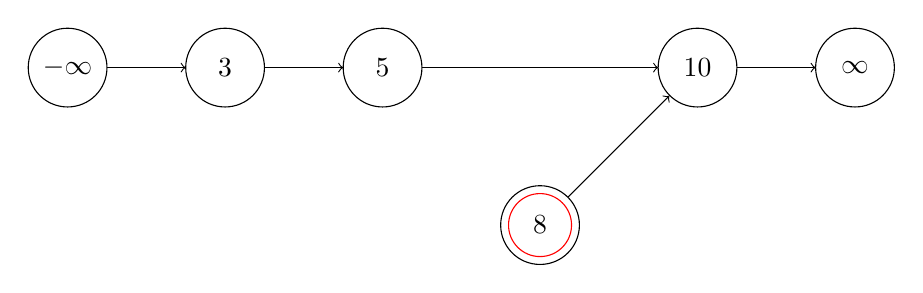
\begin{tikzpicture}
		\node[draw,circle,minimum size=1cm,inner sep=0pt] at (0,0) {$- \infty$};
		\draw[->] (0.5,0) -- (1.5,0);
		\node[draw,circle,minimum size=1cm,inner sep=0pt] at (2,0) {$3$};
		\draw[->] (2.5,0) -- (3.5,0);
		\node[draw,circle,minimum size=1cm,inner sep=0pt] at (4,0) {$5$};
        \draw[->] (4.5,0) -- (7.5,0);
        \node[draw,circle,minimum size=1cm,inner sep=0pt] (A) at (6,-2) {$8$};
        \node[draw,circle,minimum size=0.8cm,inner sep=0pt, red] at (6,-2) {};
        \node[draw,circle,minimum size=1cm,inner sep=0pt] (B) at (8,0) {$10$};
        \draw[->] (A) -- (B);
		\draw[->] (8.5,0) -- (9.5,0);
		\node[draw,circle,minimum size=1cm,inner sep=0pt] at (10,0) {$\infty$};
	\end{tikzpicture}
	\caption{fine-grained locks remove}
	\label{tik:fine-grained-remove}
\end{figure}

\begin{table}[H]
    \begin{tabularx}{\textwidth}{lX}
        \textit{add} & Gleich wie bei den fine-grained locks\\
        \textit{contains} & Die liste wird durchlaufen und bei einem erfolgreichem Fund wird sichergestellt, dass dieses Element noch nicht markiert wurde. \\
        \textit{remove} & Der Key wird gesucht und mitsamt seinem Vorgänger gesperrt. Danach wird Validiert ob dieses Element immernoch erreichbar ist. Wenn dies der Fall ist wird das Element markiert und einseitig aus der Liste entfernt, das bedeutet dass diese Node weiterhin auf den Nachfolger zeigt aber die vorherige Node wird ebenfalls auf den Nachfolger verwiesen. Dies ist in Abbildung \ref{tik:fine-grained-remove} verdeutlicht. \\
    \end{tabularx}
\end{table}

Diese Implementierung setzt Memory Management vorraus. Dies ist in Kapitel \ref{sec:mem} genauer beschrieben.

\subsection{Lock-free list-based set}

Das Ziel dieser Implementierung ist es eine Sperrungsfreie Liste zu erstellen. Dazu wird ähnlich wie bei der \textit{lazy synchronization} eine Markierung verwendet. Diese Markierung wird aber in den next-Pointer der Node integriert damit beide \textit{atomic} gelesen und geschrieben werden können. Um dies zu ermöglichen kann einfach ein Bit des Pointers genommen werden. Da bei einem 64-Bit Computer nicht alle Bits für die Adressierung des Speichers verwendet werden, kann das höchste Bit als Markierung umfunktioniert werden.

\begin{table}[H]
    \begin{tabularx}{\textwidth}{lX}
        \textit{add} & Bei add wird zuerst die der Punkt zum Einfügen gesucht und dann wird eine neue Node erzeugt die auf die nachfolger Node zeigt. Danach wird mittels \textit{compare\_exchange} der Vorgänger auf die neue Node verwiesen und somit die neue Node in die Liste eingefügt. Scheitert \textit{compare\_exchange} wird der Prozess von Neuem gestartet. \\
        \textit{contains} & Gleich wie bei \textit{lazy synchronization} \\
        \textit{remove} & Bei remove wird die zu entfernende Node zuerst gesucht und dann mittels \textit{compare\_exchange} markiert. Falls \textit{compare\_exchange} scheitert startet der Prozess wieder von vorne oder sonst wird wieder mittels \textit{compare\_exchange} versucht die Node noch aus der Liste zu entfernen indem in der Vorgänger Node der next-Pointer auf den Nachfolger gelegt wird. Falls dies jedoch scheitert werde keine werteren Versuche zum Entfernen der Node aus der Liste vorgenommen. \\
    \end{tabularx}
\end{table}
\todo{stimmt das?}

\subsubsection{Verbesserungen}
\label{subsec:impr}
In der \textit{find} Funktion wird für das Auslinken eines Nodes wird ein Compare and Swap(CAS) verwendet. Falls dies fehlschlägt, 
weil z.b. der Node zum beispiel bereits ausgelinkt wurde,
wird wieder beim Listenkopf begonnen. Um dieses Verhalten zu verbessern, wurde in \textit{Lock\_free\_impr.cpp} folgendes implementiert:\\
Es wird immer der alte \textit{predecessor} gespeichert. Sollte CAS fehlschlagen, wird überprüft ob der alte \textit{predecessor}
zum auslinken markiert wurde. Ist dies der Fall, werden \textit{predecessor, current} und \textit{successor} auf den jeweiligen Vorgänger
gesetzt und an dieser Stelle weitergemacht. 